\begin{figure*}[ht!]
    \centering
    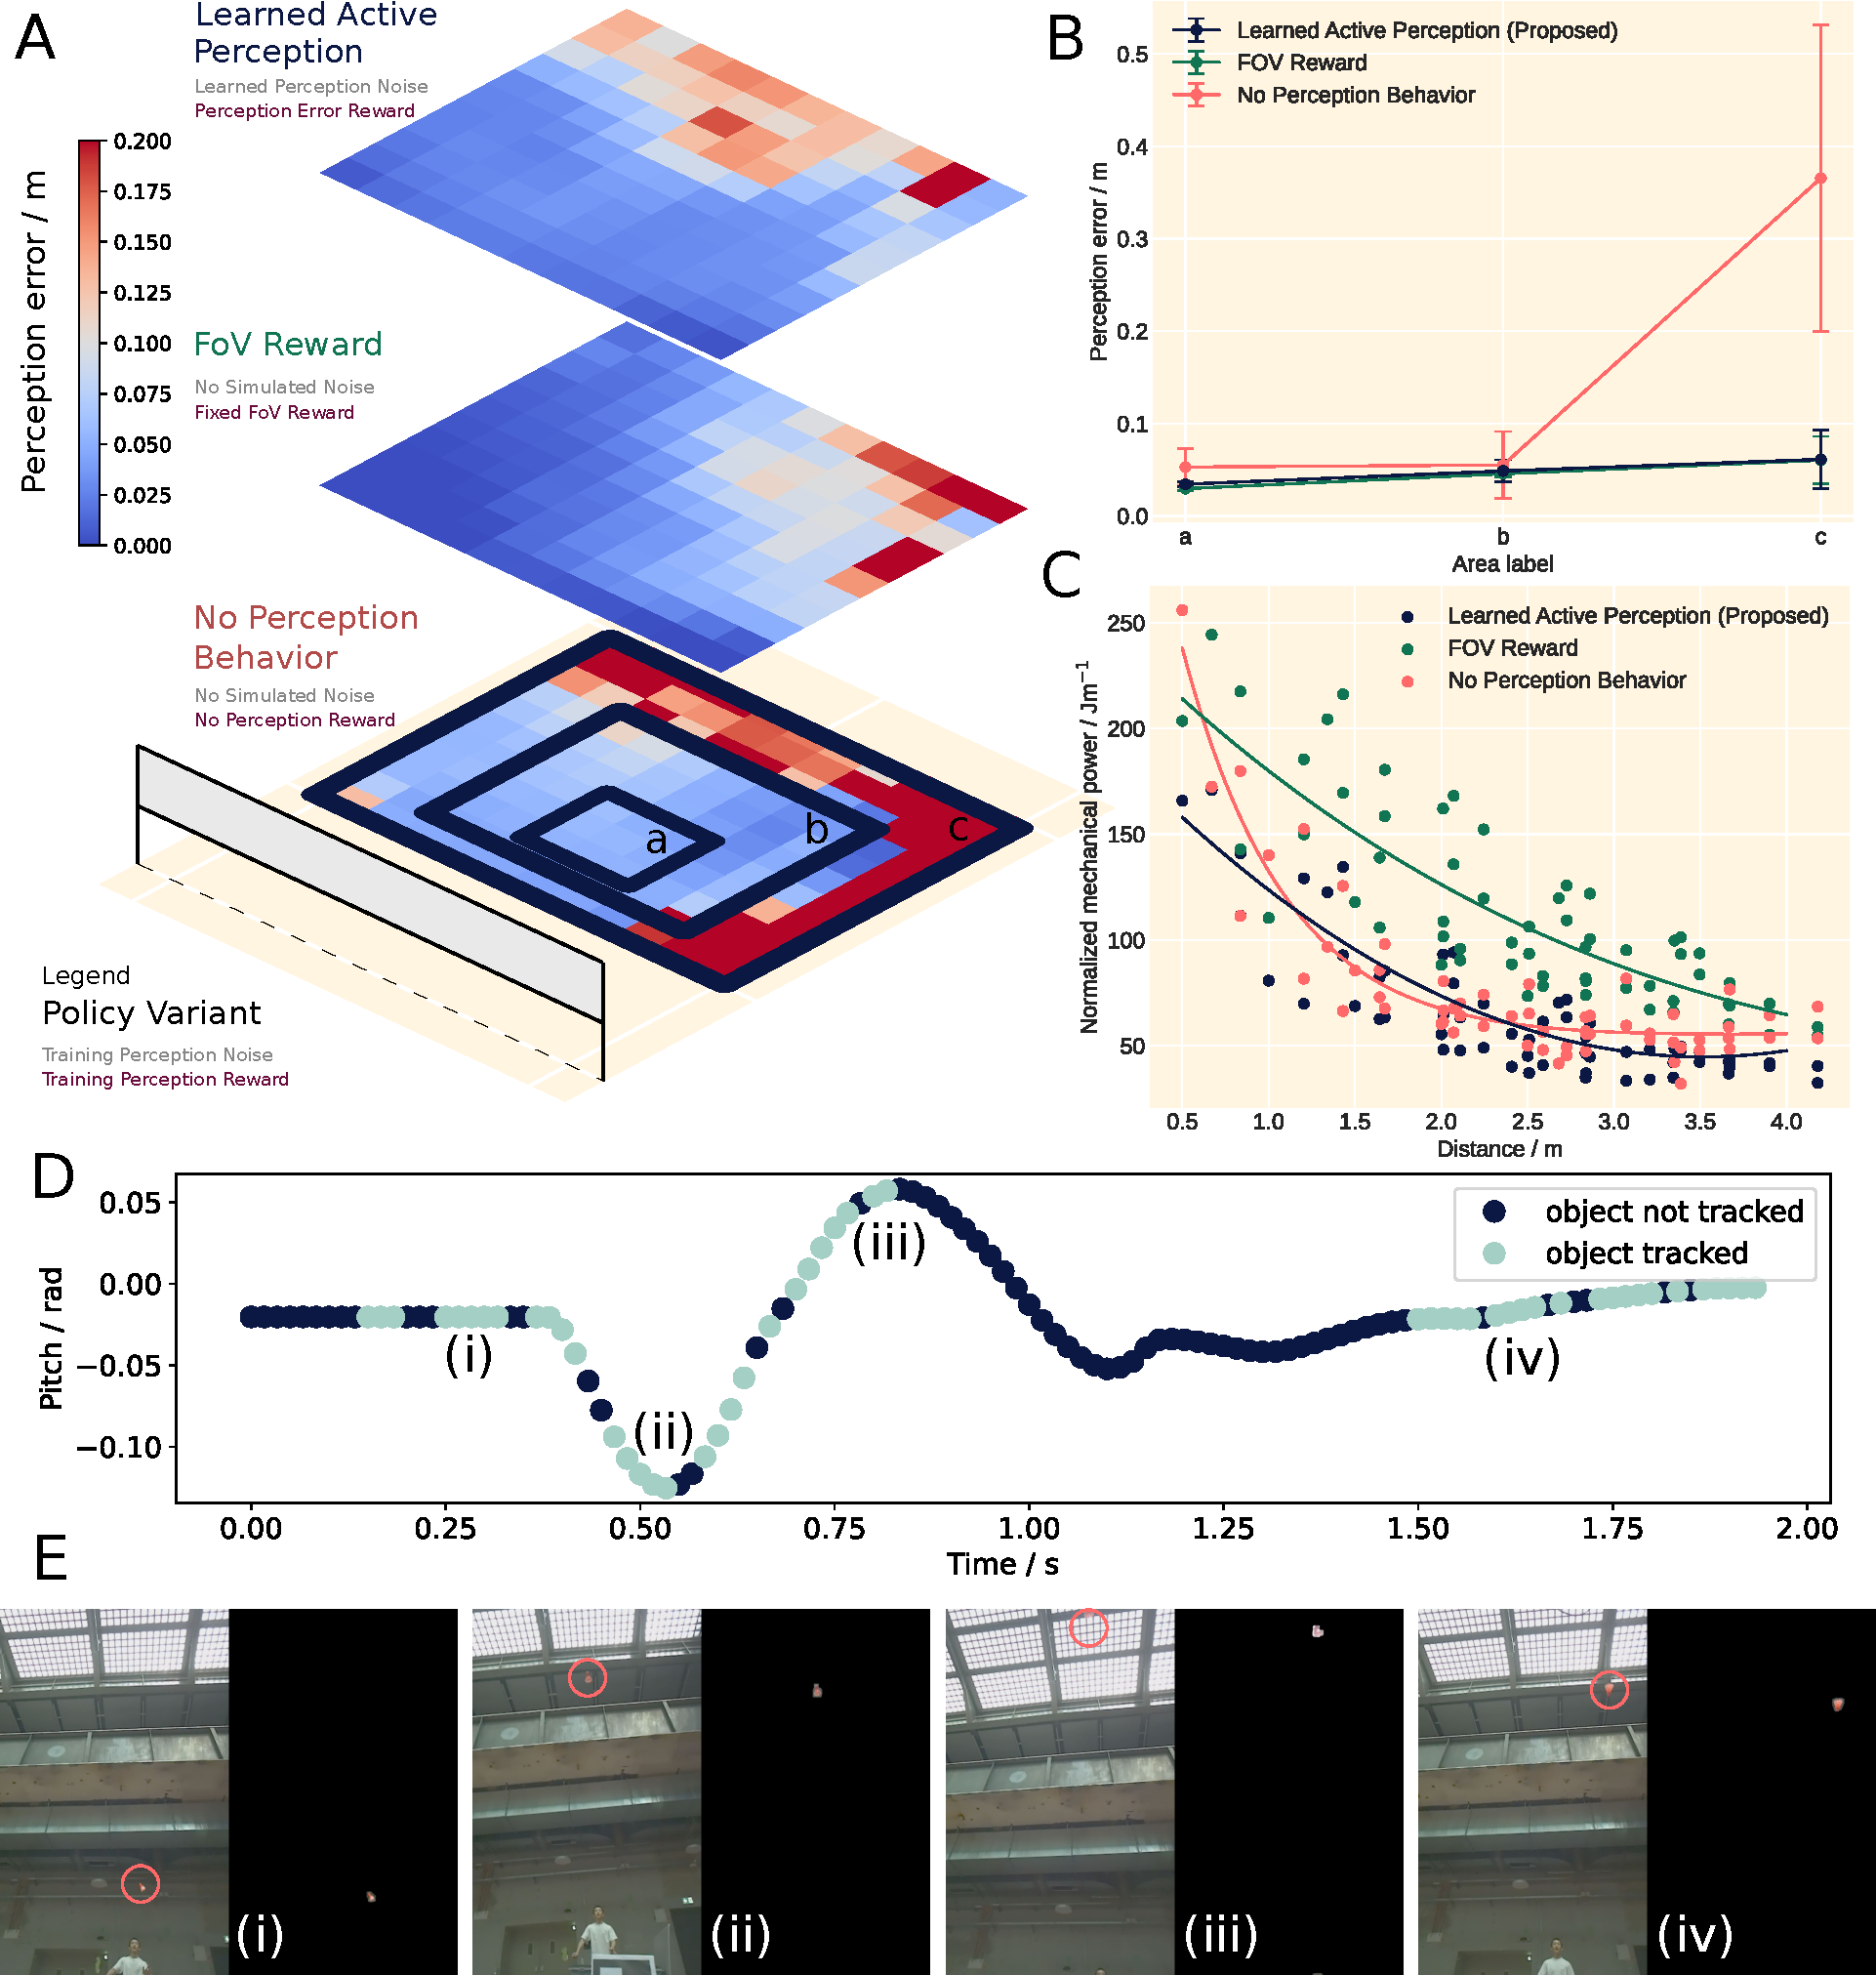
\includegraphics[width=0.9\textwidth]{Figures/ActivePerception/active_perception_pdf.pdf}
    \caption{\textbf{Learned Active Perception. (A)} A comparison of the perception error heatmap at the time of desired shuttlecock contacts. The policy trained with ground truth shuttlecock states is not incentivized to actively track the shuttlecock, leading to a larger perception error than the other two methods. The heatmaps are overlaid with the badminton court. \textbf{(B)} The perception error statistics collected based on different areas in the badminton court. The line graph shows the mean error, and the error bars represent the standard deviation, computed from 1650 trajectories per cell in each region. \textbf{(C)} The mechanical power required to execute racket swings, normalized by end-effector travel distance. Our proposed method achieves similar mechanical power efficiency to the policy trained without a perception reward, with both outperforming the FOV reward policy. The FOV reward results in inefficient base attitude and locomotion control, as it prioritizes keeping the shuttlecock within the FOV at the expense of energy efficiency.  \textbf{(D-E)} An example robot pitch trajectory during a hit. (i) ANYmal observes the shuttlecock circled in red. (ii) ANYmal pitches down while keeping the shuttlecock in the FOV. (iii) ANYmal pitches up to observe the shuttlecock for longer. (iv) ANYmal successfully hits back the shuttlecock, making it reappear in the FOV. Meanwhile, ANYmal returns to the stance posture.}
    \label{fig:active_perception}
    
    % \vspace{-1.5em}
\end{figure*}
